\documentclass[tikz,border=10pt]{standalone}
\usepackage{tikz}
\usetikzlibrary{shapes,arrows,positioning,fit,backgrounds,calc}

% Define color styles matching Mermaid classes
\tikzset{
    % Gaussian style - purple tones
    gaussian/.style={
        rectangle,
        rounded corners,
        minimum width=3cm,
        minimum height=1cm,
        text centered,
        draw=purple!70!black,
        fill=purple!10,
        line width=1.5pt,
        font=\small\bfseries
    },
    % Central style - blue tones
    central/.style={
        rectangle,
        rounded corners,
        minimum width=3cm,
        minimum height=1cm,
        text centered,
        draw=blue!70!black,
        fill=blue!10,
        line width=2pt,
        font=\small\bfseries
    },
    % Parallel style - orange tones
    parallel/.style={
        rectangle,
        rounded corners,
        minimum width=3cm,
        minimum height=1cm,
        text centered,
        draw=orange!80!black,
        fill=orange!10,
        line width=1.5pt,
        font=\small
    },
    % Symmetry style - teal tones
    symmetry/.style={
        rectangle,
        rounded corners,
        minimum width=3cm,
        minimum height=1cm,
        text centered,
        draw=teal!70!black,
        fill=teal!10,
        line width=1.5pt,
        font=\small
    },
    % External style - red tones
    external/.style={
        rectangle,
        rounded corners,
        minimum width=3cm,
        minimum height=1cm,
        text centered,
        draw=red!70!black,
        fill=red!10,
        line width=1.5pt,
        font=\small
    },
    % File style - dashed border
    file/.style={
        rectangle,
        rounded corners,
        minimum width=2.5cm,
        minimum height=1cm,
        text centered,
        draw=black!50,
        fill=white,
        line width=1pt,
        dashed,
        font=\small
    },
    % Decision diamond
    decision/.style={
        diamond,
        minimum width=2.5cm,
        minimum height=2.5cm,
        text centered,
        draw=blue!70!black,
        fill=blue!5,
        line width=1.5pt,
        font=\small,
        aspect=2
    },
    % Subgraph box style
    subgraph/.style={
        rectangle,
        draw=black!40,
        fill=gray!5,
        line width=1.5pt,
        rounded corners,
        inner sep=10pt
    },
    % Arrow style
    arrow/.style={
        ->,
        >=stealth,
        line width=1.2pt,
        draw=black!70
    },
    % Dashed arrow for info flow
    dashedarrow/.style={
        ->,
        >=stealth,
        line width=1.2pt,
        draw=black!70,
        dashed
    }
}

\begin{document}
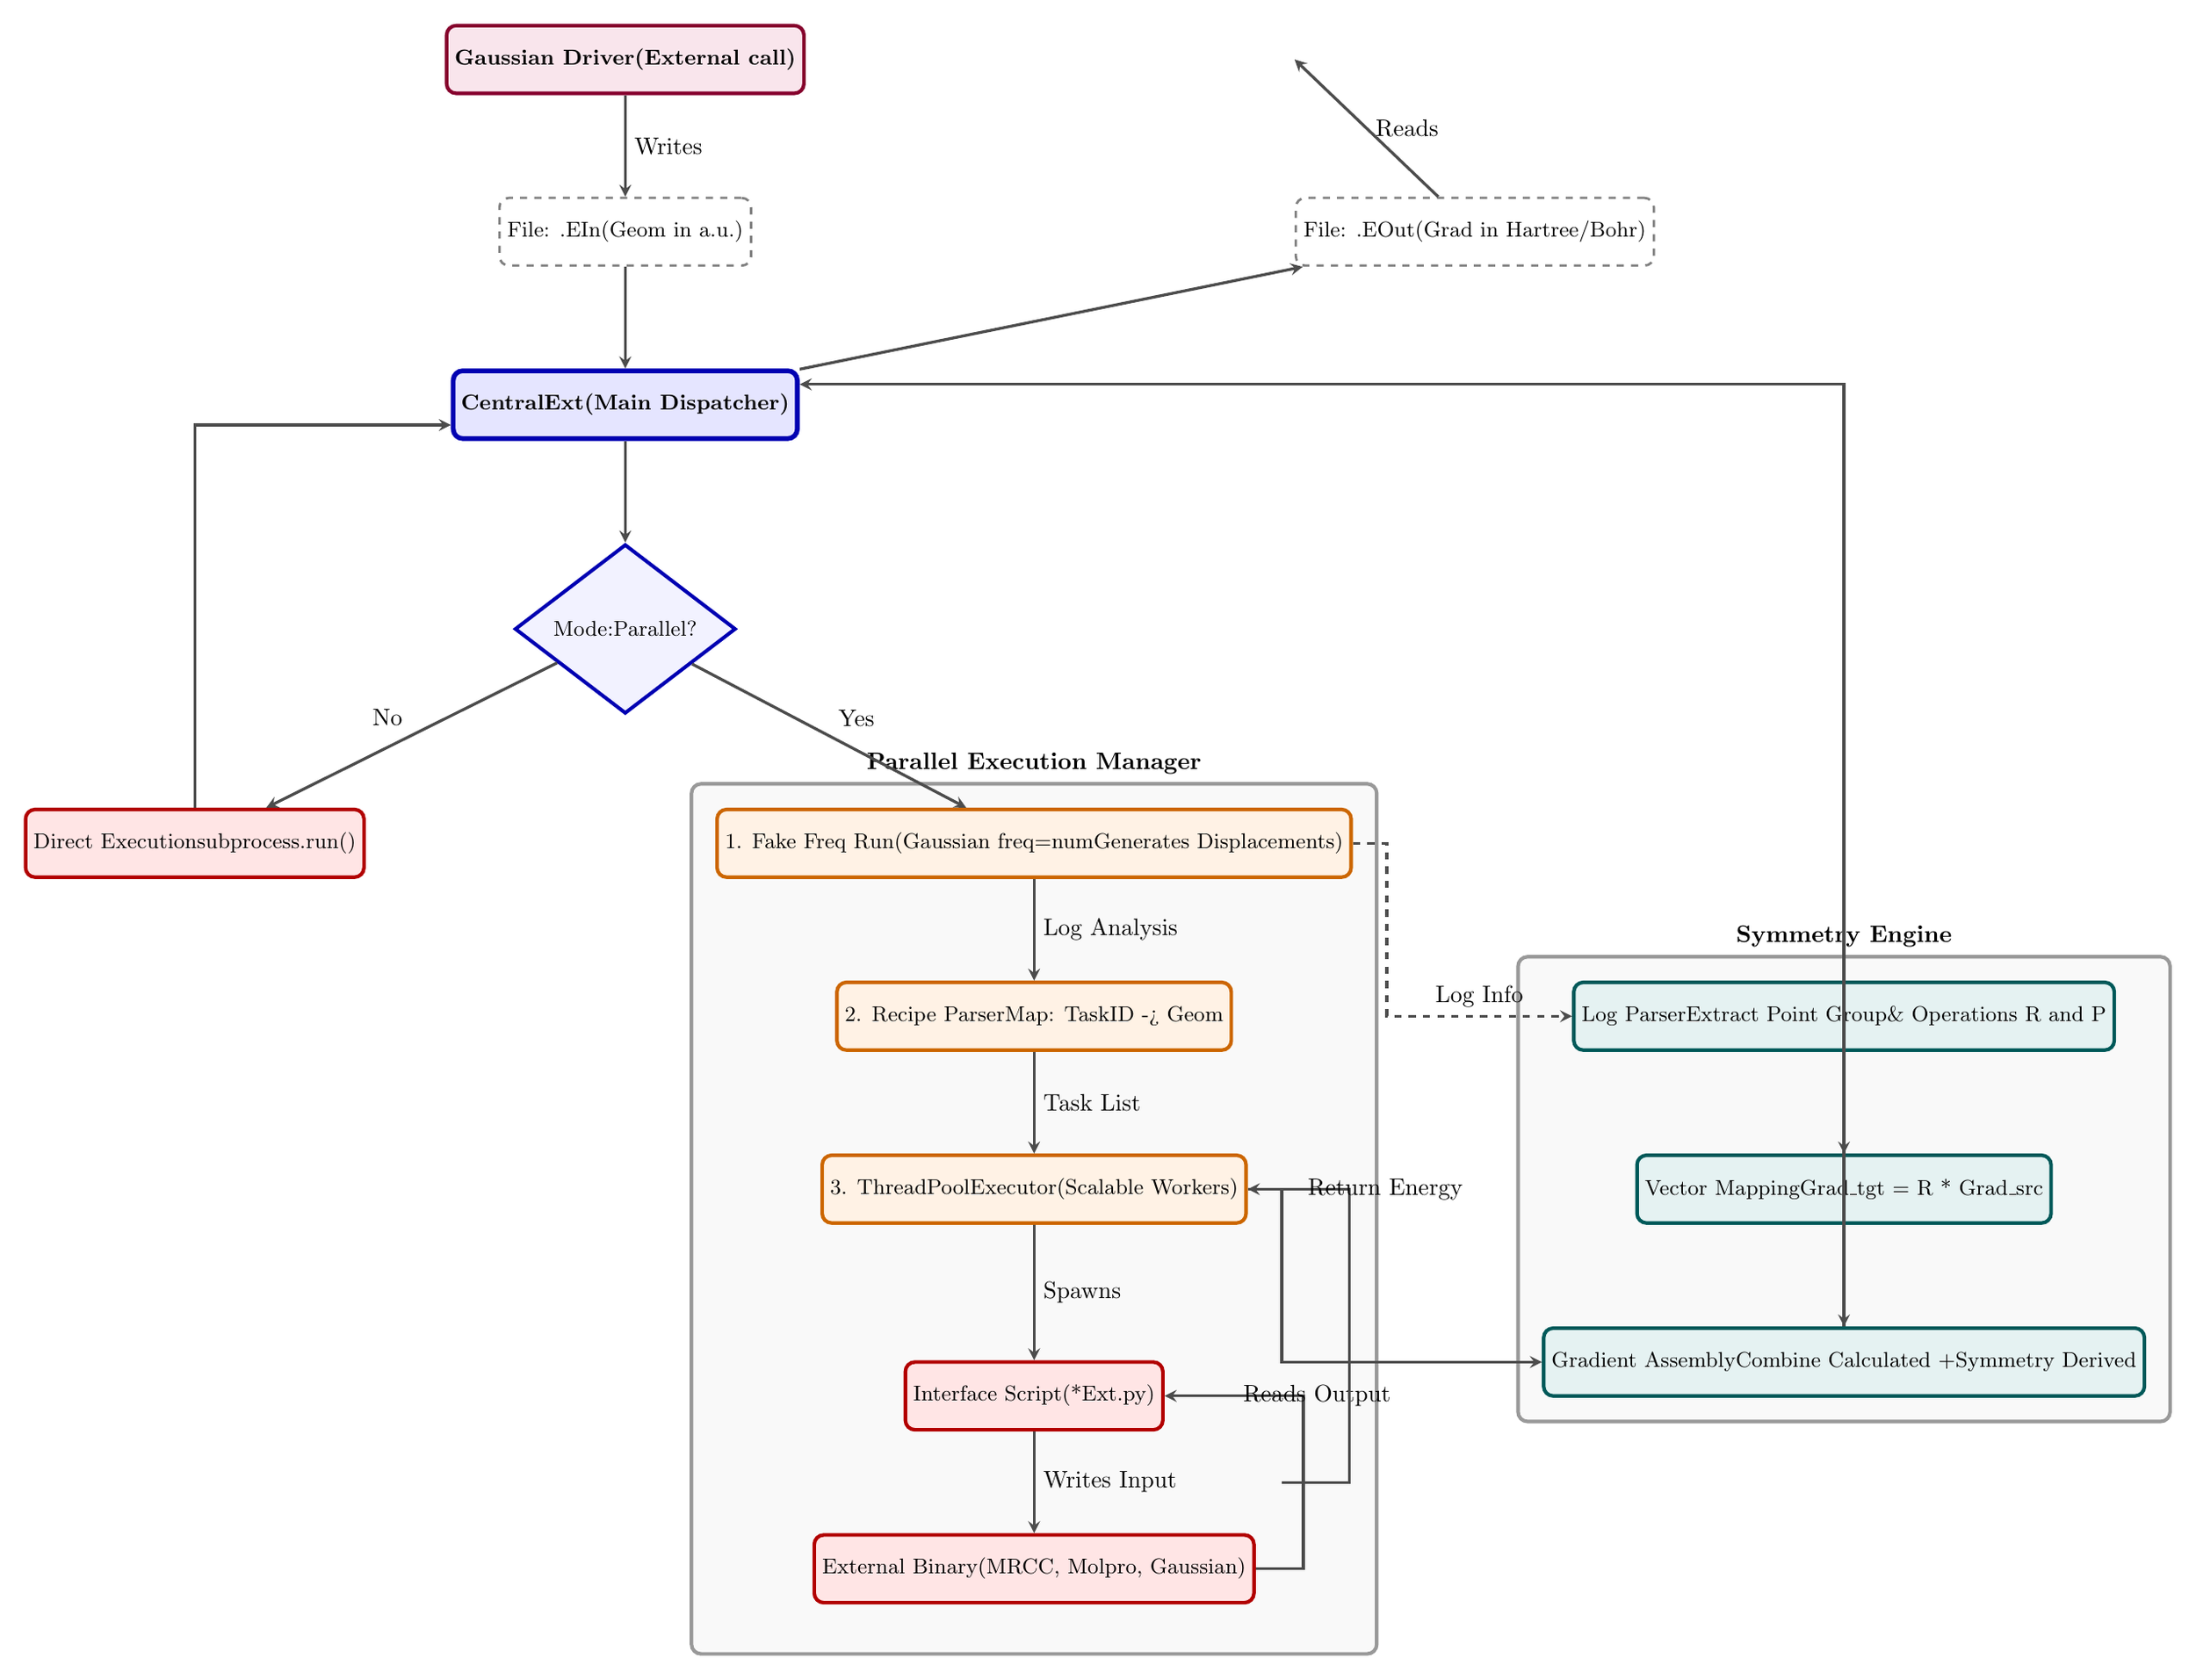
\begin{tikzpicture}[node distance=1.5cm and 2cm]

    % ========== TOP LEVEL: GAUSSIAN DRIVER ==========
    % Adjust Y-coordinate to move this section up/down
    \node[gaussian] (gdriver) at (0,0) {Gaussian Driver\\(External call)};

    % ========== FILES ==========
    % Adjust X,Y coordinates to reposition files
    \node[file, below=of gdriver] (fein) {File: .EIn\\(Geom in a.u.)};
    \node[file, right=8cm of fein] (feout) {File: .EOut\\(Grad in Hartree/Bohr)};

    % ========== CENTRAL DISPATCHER ==========
    % Adjust position to move central node
    \node[central, below=of fein] (central) {CentralExt\\(Main Dispatcher)};

    % ========== DECISION NODE ==========
    \node[decision, below=of central] (isparall) {Mode:\\Parallel?};

    % ========== SERIAL BRANCH ==========
    % Adjust X offset to move serial branch left/right
    \node[external, below left=2cm and 3cm of isparall] (serial) {Direct Execution\\subprocess.run()};

    % ========== PARALLEL BRANCH ==========
    % Parallel Manager nodes - adjust position by changing the offset values
    \node[parallel, below right=2cm and 0.5cm of isparall] (fakefreq) {1. Fake Freq Run\\(Gaussian freq=num\\Generates Displacements)};
    \node[parallel, below=of fakefreq] (recipe) {2. Recipe Parser\\Map: TaskID -> Geom};
    \node[parallel, below=of recipe] (pool) {3. ThreadPoolExecutor\\(Scalable Workers)};

    % Task Worker subgraph - adjust position relative to pool
    \node[external, below=2cm of pool] (workerscript) {Interface Script\\(*Ext.py)};
    \node[external, below=of workerscript] (binary) {External Binary\\(MRCC, Molpro, Gaussian)};

    % Task Worker box
    \begin{scope}[on background layer]
        \node[subgraph, fit=(workerscript)(binary), label=above:{\textbf{Single Task Execution}}] (taskworker) {};
    \end{scope}

    % Parallel Manager box
    \begin{scope}[on background layer]
        \node[subgraph, fit=(fakefreq)(recipe)(pool)(taskworker), label=above:{\textbf{Parallel Execution Manager}}] (parallelmgr) {};
    \end{scope}

    % ========== SYMMETRY ENGINE ==========
    % Adjust X position to move symmetry engine left/right
    \node[symmetry, right=5cm of recipe] (logparse) {Log Parser\\Extract Point Group\\\& Operations R and P};
    \node[symmetry, below=of logparse] (vectormap) {Vector Mapping\\Grad\_tgt = R * Grad\_src};
    \node[symmetry, below=of vectormap] (assembler) {Gradient Assembly\\Combine Calculated +\\Symmetry Derived};

    % Symmetry Engine box
    \begin{scope}[on background layer]
        \node[subgraph, fit=(logparse)(vectormap)(assembler), label=above:{\textbf{Symmetry Engine}}] (symmengine) {};
    \end{scope}

    % ========== CONNECTIONS ==========

    % Top flow
    \draw[arrow] (gdriver) -- node[right] {Writes} (fein);
    \draw[arrow] (fein) -- (central);
    \draw[arrow] (central) -- (isparall);

    % Decision branches
    \draw[arrow] (isparall) -- node[above left] {No} (serial);
    \draw[arrow] (isparall) -- node[above right] {Yes} (fakefreq);

    % Parallel flow
    \draw[arrow] (fakefreq) -- node[right] {Log Analysis} (recipe);
    \draw[arrow] (recipe) -- node[right] {Task List} (pool);
    \draw[arrow] (pool) -- node[right] {Spawns} (workerscript);

    % Task worker internal
    \draw[arrow] (workerscript) -- node[right] {Writes Input} (binary);
    \draw[arrow] (binary.east) -- ++(0.7,0) |- node[right, near end] {Reads Output} (workerscript.east);

    % Return from parallel
    \draw[arrow] (taskworker.east) -- ++(1,0) |- node[right, near end] {Return Energy} (pool.east);
    \draw[arrow] (pool.east) -- ++(0.5,0) |- (assembler.west);

    % Symmetry engine internal
    \draw[arrow] (logparse) -- (vectormap);
    \draw[arrow] (vectormap) -- (assembler);

    % Symmetry integration
    \draw[dashedarrow] (fakefreq.east) -- ++(0.5,0) |- node[above, near end] {Log Info} (logparse.west);
    \draw[arrow] (assembler.north) |- ($(central.east)+(0,0.3)$);

    % Serial return
    \draw[arrow] (serial.north) |- ($(central.west)+(0,-0.3)$);

    % Final output
    \draw[arrow] (central) -- (feout);
    \draw[arrow] (feout) -- node[right] {Reads} (gdriver.east -| feout.west);

\end{tikzpicture}
\end{document}
